\subsection{Yêu cầu chức năng}

Các yêu cầu chức năng được chuẩn hóa và mã hóa nhằm phục vụ quá trình thiết kế cơ sở dữ liệu, phát triển ứng dụng và kiểm thử hệ thống:

\begin{table}[H]
\centering
\small
\begin{tabularx}{\textwidth}{|l|p{3.8cm}|X|}
\hline
\textbf{Mã FR} & \textbf{Phân hệ / Chức năng} & \textbf{Mô tả chi tiết} \\ \hline
FR-01 & Quản lý truy cập \& Tài khoản & Xác thực người dùng (Đăng nhập/Đăng xuất), quản lý danh sách tài khoản và phân cấp vai trò truy cập hệ thống (Admin, Operator). \\ \hline
FR-02 & Quản lý cấu trúc nông trại & Cho phép tạo, sửa, xóa các Khu đất/Mảnh vườn (Zone); gán và quản lý thông tin các loại cây trồng tương ứng cho từng khu đất. \\ \hline
FR-03 & Quản lý danh mục thiết bị & Quản lý thông tin thiết bị (ID, định danh phần cứng, vị trí khu đất gán vào, chủng loại: cảm biến đo đạc hoặc cơ cấu chấp hành). \\ \hline
FR-04 & Nhật ký ứng dụng (Audit Log) & Ghi nhận độc lập mọi hành động của người dùng (bật/tắt thiết bị, sửa lịch trình, đổi ngưỡng cảnh báo) vào cơ sở dữ liệu nội bộ; hỗ trợ tra cứu thanh tra. \\ \hline
FR-05 & Giám sát tổng quan (Dashboard) & Hiển thị dữ liệu tổng hợp toàn hệ thống theo thời gian thực (trạng thái kết nối Online/Offline của thiết bị, số lượng khu đất, cảnh báo đang kích hoạt). \\ \hline
FR-06 & Giám sát chi tiết \& Biểu đồ & Hiển thị biểu đồ chuỗi thời gian (time-series chart) thu thập từ các thiết bị cảm biến (nhiệt độ, độ ẩm không khí, độ ẩm đất, cường độ ánh sáng). \\ \hline
FR-07 & Điều khiển thiết bị thủ công & Cho phép người vận hành gửi lệnh Bật/Tắt tức thì tới các thiết bị chấp hành (máy bơm tưới, van điện từ, đèn quang hợp, quạt thông gió). \\ \hline
FR-08 & Quản lý lịch trình tự động & Cấu hình lịch bật/tắt thiết bị định kỳ theo ngày trong tuần và khoảng thời gian trong ngày; áp dụng theo từng khu đất hoặc loại cây trồng. \\ \hline
FR-09 & Thiết lập ngưỡng \& Hành động & Cấu hình ngưỡng an toàn (Min/Max) cho từng thông số cảm biến theo loại cây; thiết lập hành động tự động kích hoạt thiết bị chấp hành đi kèm. \\ \hline
FR-10 & Tiếp nhận \& Xử lý cảnh báo & Tự động phát hiện cảm biến vượt ngưỡng, hiển thị cảnh báo đỏ thời gian thực trên giao diện và ghi nhận trạng thái xác nhận xử lý của nhân viên. \\ \hline
FR-11 & Báo cáo động \& Xuất dữ liệu & Cung cấp báo cáo chuyên biệt HTTT: phân tích đa chiều tương quan môi trường và thời lượng vận hành thiết bị, hỗ trợ lọc động và xuất tệp (CSV/Excel/PDF). \\ \hline
\end{tabularx}
\caption{Danh sách yêu cầu chức năng của hệ thống}
\label{tab:fr_list}
\end{table}

\subsection{Yêu cầu phi chức năng}

Hệ thống cần đáp ứng các tiêu chuẩn kỹ thuật phi chức năng sau nhằm đảm bảo tính ổn định, tin cậy và an toàn:

\begin{itemize}
    \item \textbf{NFR-01 (Độ trễ phản hồi - Latency):} Lệnh điều khiển thiết bị chấp hành thủ công từ giao diện người dùng tới khi thiết bị thực tế thay đổi trạng thái không vượt quá 2 giây trong điều kiện mạng ổn định.
    \item \textbf{NFR-02 (Tính toàn vẹn dữ liệu - Data Integrity):} Dữ liệu nhật ký hành động (Audit Log) được lưu trữ độc lập theo cơ chế chỉ ghi (Append-only), không cho phép chỉnh sửa hoặc xóa bởi bất kỳ người dùng nào.
    \item \textbf{NFR-03 (Khả năng chịu lỗi - Reliability):} Trong trường hợp mất kết nối Internet tạm thời giữa Gateway và Server, IoT Gateway phải lưu trữ tạm thời dữ liệu cảm biến vào bộ nhớ đệm cục bộ và tự động đồng bộ lại khi kết nối được khôi phục.
    \item \textbf{NFR-04 (Bảo mật \& Phân quyền - Security):} Toàn bộ mật khẩu người dùng phải được mã hóa bằng thuật toán băm an toàn (Bcrypt/Argon2). Hệ thống kiểm soát truy cập nghiêm ngặt theo vai trò (RBAC), ngăn chặn truy cập trái phép vào các API cấu hình.
\end{itemize}

\subsection{Mô hình Tác nhân và Danh mục Use Case}

\textbf{1. Danh sách tác nhân hệ thống (Actors):}
\begin{itemize}
    \item \textbf{Quản trị viên (Admin):} Đại diện cho nhóm người dùng quản trị kỹ thuật, chịu trách nhiệm quản lý tài khoản người dùng, phân quyền, thiết lập danh mục hạ tầng nông trại (khu đất, cây trồng, thiết bị) và tra cứu nhật ký ứng dụng.
    \item \textbf{Người vận hành (Operator):} Đại diện cho nhân viên nông trại trực tiếp vận hành hệ thống, thực hiện giám sát thông số thời gian thực, điều khiển thiết bị, cấu hình lịch trình/ngưỡng an toàn và khai thác báo cáo phân tích.
\end{itemize}

\vspace{0.3cm}
\noindent\textbf{2. Danh mục phân rã Use Case theo 4 phân hệ:}
\begin{itemize}
    \item \textbf{Phân hệ Quản trị \& Kiểm toán (Admin):}
    \begin{itemize}
        \item UC-01: Đăng nhập / Đăng xuất hệ thống
        \item UC-02: Quản lý người dùng \& Phân quyền
        \item UC-03: Quản lý Khu đất \& Loại cây trồng
        \item UC-04: Quản lý danh mục \& Thiết bị
        \item UC-05: Tra cứu nhật ký ứng dụng (Audit Log)
    \end{itemize}
    \item \textbf{Phân hệ Giám sát \& Điều khiển:}
    \begin{itemize}
        \item UC-06: Xem Dashboard tổng hợp toàn hệ thống
        \item UC-07: Giám sát dữ liệu \& Biểu đồ cảm biến
        \item UC-08: Điều khiển thiết bị chấp hành thủ công
    \end{itemize}
    \item \textbf{Phân hệ Tự động hóa \& Cảnh báo:}
    \begin{itemize}
        \item UC-09: Cấu hình lịch trình hoạt động thiết bị
        \item UC-10: Thiết lập ngưỡng \& Hành động
        \item UC-11: Tiếp nhận \& Xử lý cảnh báo
    \end{itemize}
    \item \textbf{Phân hệ Báo cáo \& Phân tích (HTTT):}
    \begin{itemize}
        \item UC-12: Khai thác báo cáo đa chiều \& Xuất dữ liệu
    \end{itemize}
\end{itemize}

\subsection{Sơ đồ và Ma trận phân nhiệm Use Case}

Sơ đồ Use Case tổng thể của hệ thống được minh họa tại Hình~\ref{fig:usecase_diagram}. Ranh giới hệ thống phân định rõ 12 Use Case phân bổ trong 4 phân hệ cùng các luồng kích hoạt từ hai nhóm tác nhân Quản trị viên và Người vận hành.

\begin{figure}[H]
    \centering
    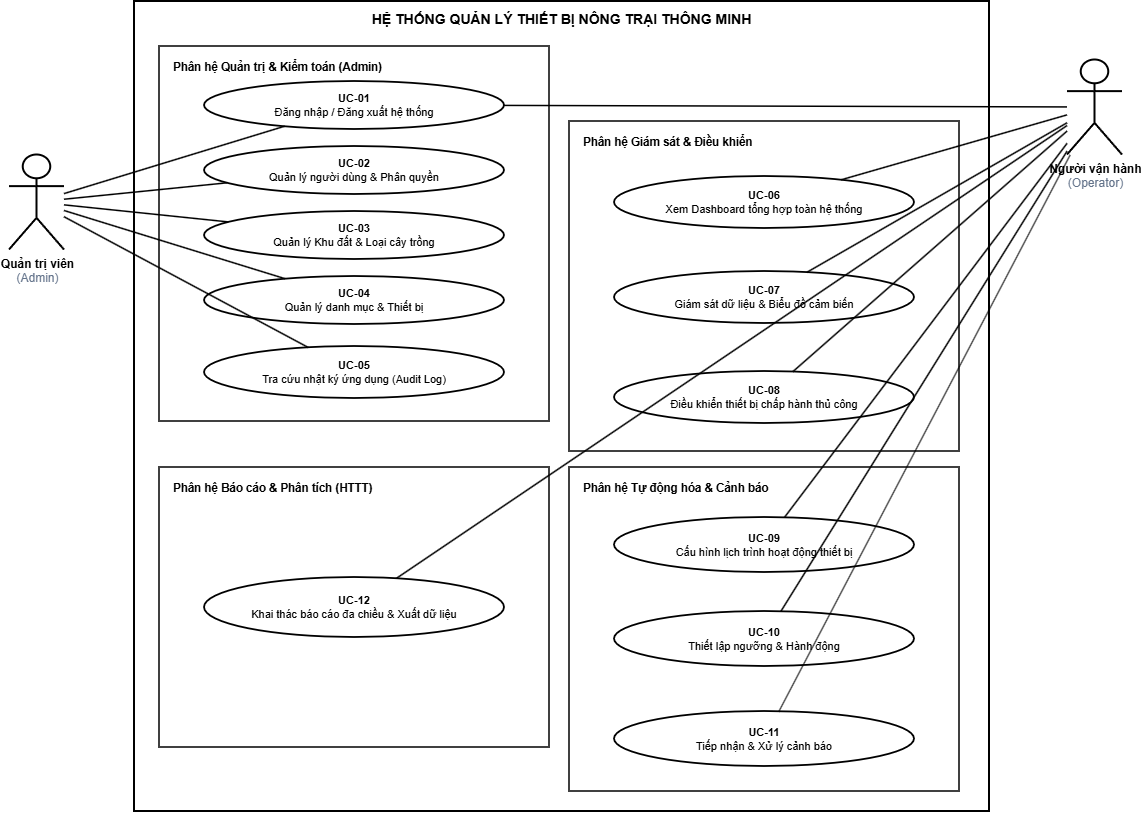
\includegraphics[width=1\textwidth]{images/usecase_diagram.png}
    \caption{Sơ đồ Use Case tổng thể Hệ thống Quản lý Thiết bị Nông trại Thông minh}
    \label{fig:usecase_diagram}
\end{figure}

Sự phân bổ trách nhiệm và quyền hạn truy cập chức năng của các tác nhân được tổng hợp thông qua Ma trận phân nhiệm Use Case tại Bảng~\ref{tab:traceability_matrix}:

\begin{table}[H]
\centering
\small
\begin{tabularx}{\textwidth}{|l|X|>{\centering\arraybackslash}p{2.5cm}|>{\centering\arraybackslash}p{2.5cm}|}
\hline
\textbf{Mã UC} & \textbf{Tên Use Case} & \textbf{Quản trị viên (Admin)} & \textbf{Người vận hành (Operator)} \\ \hline
UC-01 & Đăng nhập / Đăng xuất hệ thống & $\bullet$ & $\bullet$ \\ \hline
UC-02 & Quản lý người dùng \& Phân quyền & $\bullet$ & \\ \hline
UC-03 & Quản lý Khu đất \& Loại cây trồng & $\bullet$ & \\ \hline
UC-04 & Quản lý danh mục \& Thiết bị & $\bullet$ & \\ \hline
UC-05 & Tra cứu nhật ký ứng dụng (Audit Log) & $\bullet$ & \\ \hline
UC-06 & Xem Dashboard tổng hợp toàn hệ thống & $\bullet$ & $\bullet$ \\ \hline
UC-07 & Giám sát dữ liệu \& Biểu đồ cảm biến & & $\bullet$ \\ \hline
UC-08 & Điều khiển thiết bị chấp hành thủ công & & $\bullet$ \\ \hline
UC-09 & Cấu hình lịch trình hoạt động thiết bị & & $\bullet$ \\ \hline
UC-10 & Thiết lập ngưỡng \& Hành động & & $\bullet$ \\ \hline
UC-11 & Tiếp nhận \& Xử lý cảnh báo & & $\bullet$ \\ \hline
UC-12 & Khai thác báo cáo đa chiều \& Xuất dữ liệu & $\bullet$ & $\bullet$ \\ \hline
\end{tabularx}
\caption{Ma trận phân nhiệm vai trò và Use Case trong hệ thống}
\label{tab:traceability_matrix}
\end{table}

\subsection{Đặc tả Use Case chi tiết}

Dưới đây là các bảng đặc tả chi tiết cho các Use Case nghiệp vụ nòng cốt đại diện cho từng phân hệ của hệ thống.

% --- UC-05 ---
\begin{table}[H]
\centering
\small
\begin{tabularx}{\textwidth}{|p{3.2cm}|X|}
\hline
\textbf{Mục} & \textbf{Nội dung đặc tả} \\ \hline
\textbf{Mã Use Case} & \textbf{UC-05} \\ \hline
\textbf{Tên Use Case} & \textbf{Tra cứu nhật ký ứng dụng (Audit Log)} \\ \hline
\textbf{Tác nhân chính} & Quản trị viên (Admin) \\ \hline
\textbf{Mô tả ngắn} & Cho phép Quản trị viên tra cứu, tìm kiếm và thanh tra lịch sử các hành động can thiệp hệ thống của người dùng (đổi ngưỡng, sửa lịch, bật/tắt thủ công). \\ \hline
\textbf{Tiền điều kiện} & Quản trị viên đã đăng nhập thành công vào hệ thống. \\ \hline
\textbf{Hậu điều kiện} & Danh sách các bản ghi nhật ký tương ứng được hiển thị trên giao diện theo đúng tiêu chí tìm kiếm. \\ \hline
\textbf{Luồng sự kiện chính} & 
\begin{enumerate}[leftmargin=*, nosep]
    \item Quản trị viên truy cập vào menu \textit{Quản lý nhật ký ứng dụng}.
    \item Hệ thống hiển thị giao diện bộ lọc gồm: khoảng thời gian, loại hành động, mã nhân viên thao tác và mã thiết bị bị tác động.
    \item Quản trị viên thiết lập các tiêu chí lọc cần tra cứu và nhấn nút \textit{Tìm kiếm}.
    \item Hệ thống truy vấn bảng cơ sở dữ liệu nhật ký nội bộ (Audit Log Table) và hiển thị kết quả phân trang dạng danh sách.
    \item Quản trị viên có thể nhấp chọn từng dòng bản ghi để xem chi tiết thông số cũ và thông số mới được thay đổi.
\end{enumerate} \\ \hline
\textbf{Luồng ngoại lệ} & 
\begin{itemize}[leftmargin=*, nosep]
    \item \textbf{4a. Không tìm thấy kết quả phù hợp:} Hệ thống hiển thị thông báo không có bản ghi nào thỏa mãn điều kiện và hướng dẫn làm mới bộ lọc.
\end{itemize} \\ \hline
\end{tabularx}
\caption{Đặc tả Use Case UC-05: Tra cứu nhật ký ứng dụng (Audit Log)}
\label{tab:uc_05}
\end{table}

% --- UC-08 ---
\begin{table}[H]
\centering
\small
\begin{tabularx}{\textwidth}{|p{3.2cm}|X|}
\hline
\textbf{Mục} & \textbf{Nội dung đặc tả} \\ \hline
\textbf{Mã Use Case} & \textbf{UC-08} \\ \hline
\textbf{Tên Use Case} & \textbf{Điều khiển thiết bị chấp hành thủ công} \\ \hline
\textbf{Tác nhân chính} & Người vận hành (Operator) \\ \hline
\textbf{Mô tả ngắn} & Người vận hành gửi lệnh Bật/Tắt tức thì tới các thiết bị cơ cấu chấp hành (bơm, van tưới, đèn, quạt) từ giao diện Web/App. \\ \hline
\textbf{Tiền điều kiện} & Người dùng đã đăng nhập; thiết bị chấp hành đang ở trạng thái Online và sẵn sàng nhận lệnh. \\ \hline
\textbf{Hậu điều kiện} & Trạng thái hoạt động của thiết bị thay đổi ngoài thực tế; hệ thống tự động lưu một bản ghi tác động vào bảng Audit Log. \\ \hline
\textbf{Luồng sự kiện chính} & 
\begin{enumerate}[leftmargin=*, nosep]
    \item Người vận hành chọn Khu đất và chọn thiết bị chấp hành cần điều khiển.
    \item Người vận hành gạt công tắc Bật/Tắt trên giao diện giám sát.
    \item Hệ thống gửi thông điệp điều khiển xuống thiết bị thông qua giao thức MQTT.
    \item Thiết bị chấp hành thay đổi trạng thái rơ-le và gửi bản tin phản hồi xác nhận (ACK).
    \item Hệ thống cập nhật trạng thái hiển thị mới trên giao diện người dùng.
    \item Hệ thống tự động lưu vết sự kiện điều khiển vào bảng nhật ký ứng dụng (User ID, Device ID, Lệnh điều khiển, Thời gian thực hiện).
\end{enumerate} \\ \hline
\textbf{Luồng ngoại lệ} & 
\begin{itemize}[leftmargin=*, nosep]
    \item \textbf{4a. Quá thời gian phản hồi (Timeout):} Nếu sau 2 giây không nhận được xác nhận từ thiết bị, giao diện khôi phục lại công tắc về trạng thái ban đầu và hiển thị thông báo: \textit{"Không thể kết nối đến thiết bị"}.
\end{itemize} \\ \hline
\end{tabularx}
\caption{Đặc tả Use Case UC-08: Điều khiển thiết bị chấp hành thủ công}
\label{tab:uc_08}
\end{table}

% --- UC-09 ---
\begin{table}[H]
\centering
\small
\begin{tabularx}{\textwidth}{|p{3.2cm}|X|}
\hline
\textbf{Mục} & \textbf{Nội dung đặc tả} \\ \hline
\textbf{Mã Use Case} & \textbf{UC-09} \\ \hline
\textbf{Tên Use Case} & \textbf{Cấu hình lịch trình hoạt động thiết bị} \\ \hline
\textbf{Tác nhân chính} & Người vận hành (Operator) \\ \hline
\textbf{Mô tả ngắn} & Thiết lập lịch trình bật/tắt tự động theo chu kỳ ngày trong tuần và khung giờ trong ngày cho thiết bị chấp hành gắn với từng khu đất và loại cây. \\ \hline
\textbf{Tiền điều kiện} & Người dùng đã xác thực; khu đất, cây trồng và thiết bị đã được cấu hình trên hệ thống. \\ \hline
\textbf{Hậu điều kiện} & Lịch trình mới được lưu trữ và kích hoạt trong tiến trình lập lịch tự động của hệ thống. \\ \hline
\textbf{Luồng sự kiện chính} & 
\begin{enumerate}[leftmargin=*, nosep]
    \item Người vận hành truy cập menu \textit{Quản lý lịch trình}.
    \item Hệ thống hiển thị danh sách các lịch trình hiện hành theo từng Khu đất / Cây trồng.
    \item Người dùng nhấn nút \textit{Tạo lịch trình mới}.
    \item Người dùng chọn Khu đất, chọn thiết bị áp dụng, chu kỳ ngày hoạt động và khung giờ kích hoạt (giờ bật, thời lượng chạy).
    \item Người dùng nhấn nút \textit{Lưu cấu hình}.
    \item Hệ thống kiểm tra tính hợp lệ dữ liệu và kiểm tra xung đột thời gian với các lịch trình đã tồn tại trên thiết bị.
    \item Hệ thống lưu lịch trình vào cơ sở dữ liệu, tự động ghi nhận hành động vào Audit Log và thông báo thành công.
\end{enumerate} \\ \hline
\textbf{Luồng ngoại lệ} & 
\begin{itemize}[leftmargin=*, nosep]
    \item \textbf{6a. Xung đột khung giờ hoạt động:} Nếu thiết bị đã có lịch trình khác chạy trong cùng khoảng thời gian, hệ thống báo lỗi xung đột và yêu cầu người dùng chọn lại thời gian.
    \item \textbf{6b. Bỏ trống trường bắt buộc:} Hệ thống đánh dấu đỏ các trường bị thiếu và yêu cầu người dùng bổ sung đầy đủ.
\end{itemize} \\ \hline
\end{tabularx}
\caption{Đặc tả Use Case UC-09: Cấu hình lịch trình hoạt động thiết bị}
\label{tab:uc_09}
\end{table}

% --- UC-10 ---
\begin{table}[H]
\centering
\small
\begin{tabularx}{\textwidth}{|p{3.2cm}|X|}
\hline
\textbf{Mục} & \textbf{Nội dung đặc tả} \\ \hline
\textbf{Mã Use Case} & \textbf{UC-10} \\ \hline
\textbf{Tên Use Case} & \textbf{Thiết lập ngưỡng \& Hành động} \\ \hline
\textbf{Tác nhân chính} & Người vận hành (Operator) \\ \hline
\textbf{Mô tả ngắn} & Cài đặt dải giá trị môi trường an toàn theo loại cây trồng và cấu hình hành động tự động kích hoạt thiết bị khi phát hiện vi phạm ngưỡng. \\ \hline
\textbf{Tiền điều kiện} & Cảm biến giám sát và thiết bị chấp hành mục tiêu đang hoạt động bình thường trên hệ thống. \\ \hline
\textbf{Hậu điều kiện} & Quy tắc (Rule) được kích hoạt và đưa vào tiến trình kiểm tra dữ liệu chuỗi thời gian của cảm biến. \\ \hline
\textbf{Luồng sự kiện chính} & 
\begin{enumerate}[leftmargin=*, nosep]
    \item Người vận hành truy cập phân hệ \textit{Cài đặt ngưỡng an toàn}.
    \item Chọn Khu đất và Loại cây trồng cần thiết lập.
    \item Nhấn nút \textit{Thêm quy tắc mới}.
    \item Chọn loại cảm biến đo (độ ẩm đất, nhiệt độ) và cài đặt điều kiện biên (ví dụ: Độ ẩm đất $<$ 45\%).
    \item Cấu hình hành động đi kèm (ví dụ: Tự động bật máy bơm tưới trong thời gian 15 phút).
    \item Người dùng nhấn nút \textit{Lưu quy tắc}.
    \item Hệ thống kiểm tra tính hợp lệ số học, lưu quy tắc vào cơ sở dữ liệu, ghi log thao tác và hiển thị thông báo hoàn tất.
\end{enumerate} \\ \hline
\textbf{Luồng ngoại lệ} & 
\begin{itemize}[leftmargin=*, nosep]
    \item \textbf{6a. Ngưỡng số học phi logic:} Nếu người dùng nhập cận dưới lớn hơn cận trên ($Min > Max$), hệ thống báo lỗi và yêu cầu điều chỉnh lại giá trị.
\end{itemize} \\ \hline
\end{tabularx}
\caption{Đặc tả Use Case UC-10: Thiết lập ngưỡng \& Hành động}
\label{tab:uc_10}
\end{table}

% --- UC-11 ---
\begin{table}[H]
\centering
\small
\begin{tabularx}{\textwidth}{|p{3.2cm}|X|}
\hline
\textbf{Mục} & \textbf{Nội dung đặc tả} \\ \hline
\textbf{Mã Use Case} & \textbf{UC-11} \\ \hline
\textbf{Tên Use Case} & \textbf{Tiếp nhận \& Xử lý cảnh báo} \\ \hline
\textbf{Tác nhân chính} & Người vận hành (Operator) \\ \hline
\textbf{Mô tả ngắn} & Hệ thống tự động phát cảnh báo khi số liệu môi trường vượt ngưỡng cho phép; người vận hành tiếp nhận thông báo và ghi nhận kết quả xử lý thực địa. \\ \hline
\textbf{Tiền điều kiện} & Quy tắc ngưỡng (UC-10) đã được kích hoạt; cảm biến đang truyền nhận dữ liệu định kỳ. \\ \hline
\textbf{Hậu điều kiện} & Bản ghi sự cố được lưu trữ; trạng thái cảnh báo chuyển từ \textit{"Đang xử lý"} sang \textit{"Đã giải quyết"}. \\ \hline
\textbf{Luồng sự kiện chính} & 
\begin{enumerate}[leftmargin=*, nosep]
    \item Dữ liệu cảm biến mới gửi về hệ thống vi phạm quy tắc ngưỡng an toàn đã cài đặt.
    \item Hệ thống kích hoạt hành động tự động liên kết (nếu có) và hiển thị thông báo cảnh báo đỏ trên giao diện Dashboard.
    \item Người vận hành nhấp vào biểu tượng cảnh báo để xem thông tin chi tiết (vị trí khu đất, chỉ số đo, thời gian phát hiện).
    \item Người vận hành kiểm tra tình hình thực địa tại nông trại và thực hiện các biện pháp can thiệp cần thiết.
    \item Người vận hành nhấn nút \textit{Xác nhận đã xử lý} trên giao diện và nhập ghi chú khắc phục sự cố.
    \item Hệ thống cập nhật trạng thái sự cố thành \textit{"Đã giải quyết"} và ghi nhận thời gian phản hồi của nhân viên.
\end{enumerate} \\ \hline
\textbf{Luồng ngoại lệ} & 
\begin{itemize}[leftmargin=*, nosep]
    \item \textbf{2a. Kích hoạt hành động tự động thất bại:} Nếu việc tự động bật thiết bị đi kèm không nhận được xác nhận từ rơ-le, hệ thống nâng mức cảnh báo thành \textit{"Khẩn cấp (Critical)"} yêu cầu can thiệp thủ công ngay lập tức.
\end{itemize} \\ \hline
\end{tabularx}
\caption{Đặc tả Use Case UC-11: Tiếp nhận \& Xử lý cảnh báo}
\label{tab:uc_11}
\end{table}

% --- UC-12 ---
\begin{table}[H]
\centering
\small
\begin{tabularx}{\textwidth}{|p{3.2cm}|X|}
\hline
\textbf{Mục} & \textbf{Nội dung đặc tả} \\ \hline
\textbf{Mã Use Case} & \textbf{UC-12} \\ \hline
\textbf{Tên Use Case} & \textbf{Khai thác báo cáo đa chiều \& Xuất dữ liệu} \\ \hline
\textbf{Tác nhân chính} & Người vận hành (Operator), Quản trị viên (Admin) \\ \hline
\textbf{Mô tả ngắn} & Cung cấp công cụ phân tích dữ liệu chuyên biệt của Hệ thống thông tin (HTTT), cho phép lọc dữ liệu đa chiều, trực quan hóa biểu đồ và xuất tệp phục vụ lưu trữ, báo cáo định kỳ. \\ \hline
\textbf{Tiền điều kiện} & Hệ thống đã tích lũy dữ liệu cảm biến và lịch sử vận hành trong cơ sở dữ liệu. \\ \hline
\textbf{Hậu điều kiện} & Báo cáo tổng hợp được hiển thị trên giao diện hoặc tệp dữ liệu được tải về máy tính người dùng. \\ \hline
\textbf{Luồng sự kiện chính} & 
\begin{enumerate}[leftmargin=*, nosep]
    \item Người dùng truy cập phân hệ \textit{Báo cáo \& Phân tích}.
    \item Thiết lập các chiều lọc dữ liệu: Khoảng thời gian (tuần/tháng/vụ mùa), danh sách Khu đất, Loại cây trồng, loại thông số phân tích (nhiệt độ, độ ẩm, thời lượng bơm chạy).
    \item Chọn định dạng hiển thị trực quan (Biểu đồ đường, Biểu đồ cột tổng hợp hoặc Bảng số liệu chi tiết).
    \item Người dùng nhấn nút \textit{Tạo báo cáo}.
    \item Hệ thống thực hiện tính toán tổng hợp dữ liệu (Trung bình, Cực đại, Cực tiểu, Tổng thời gian vận hành) và dựng báo cáo trực quan trên màn hình.
    \item Người dùng chọn định dạng xuất tệp mong muốn (CSV, Excel hoặc PDF) và nhấn nút \textit{Tải xuống}.
    \item Hệ thống đóng gói dữ liệu và tự động tải tệp tin về thiết bị người dùng.
\end{enumerate} \\ \hline
\textbf{Luồng ngoại lệ} & 
\begin{itemize}[leftmargin=*, nosep]
    \item \textbf{5a. Khoảng thời gian không có dữ liệu:} Hệ thống hiển thị thông báo trạng thái rỗng (Empty State) và đề xuất người dùng mở rộng phạm vi thời gian tìm kiếm.
\end{itemize} \\ \hline
\end{tabularx}
\caption{Đặc tả Use Case UC-12: Khai thác báo cáo đa chiều \& Xuất dữ liệu}
\label{tab:uc_12}
\end{table}